\documentclass{article}
\usepackage{tikz}
\usetikzlibrary{arrows.meta,positioning,calc,shapes.geometric}
\pagestyle{empty}
\begin{document}
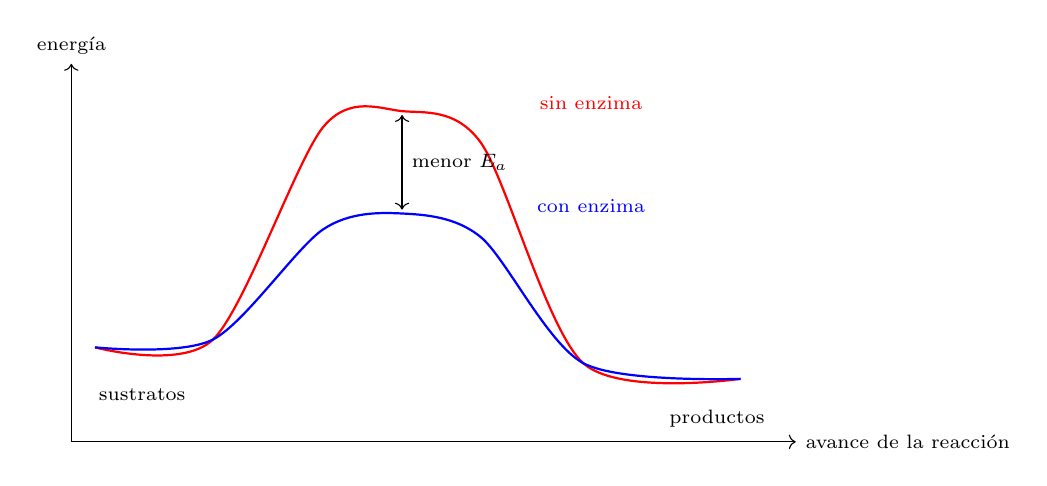
\begin{tikzpicture}

\draw[->] (0,0) -- (0,4.8) node[above, font=\scriptsize] {energía}; \draw[->] (0,0) -- (9.2,0) node[right, font=\scriptsize] {avance de la reacción};
\draw[thick, red] plot[smooth] coordinates {(0.3,1.2) (1.8,1.3) (3.2,4.0) (4.2,4.2) (5.2,3.8) (6.5,1.0) (8.5,0.8)};
\draw[thick, blue] plot[smooth] coordinates {(0.3,1.2) (1.8,1.3) (3.2,2.7) (4.2,2.9) (5.2,2.6) (6.5,1.0) (8.5,0.8)};
\node[red, font=\scriptsize] at (6.6,4.3) {sin enzima}; \node[blue, font=\scriptsize] at (6.6,3.0) {con enzima};
\draw[<->] (4.2,2.95) -- (4.2,4.15) node[midway, right, font=\scriptsize] {menor $E_a$};
\node[font=\scriptsize] at (0.9,0.6) {sustratos}; \node[font=\scriptsize] at (8.2,0.3) {productos};

\end{tikzpicture}
\end{document}
